\documentclass[10pt,a4paper]{amsart}
\usepackage[margin=19mm]{geometry}
\usepackage{amsmath,amssymb,mathtools}
\usepackage[scr=rsfs,cal=euler]{mathalfa}
\usepackage{xfrac}
\usepackage[unicode,hidelinks,bookmarks=false]{hyperref}
\newcommand{\ie}{i.e.\ }
\newcommand{\cf}{cf.\ }
\newcommand{\resp}{respectively\ }
\newcommand{\Subsection}{\subsection}
\providecommand{\nobreakdash}{\nobreak\hbox{-}}
\setlength{\emergencystretch}{2em}
\multlinegap0pt
\usepackage{tikz}
\usepackage{amssymb}
\usepackage{mathtools}
\newtheorem{lemma}{Lemma}
\newtheorem{theorem}{Theorem}
\title{\textbf{Best approximation of a three-variable function by sum of one-variable coordinate functions}}
\author{Rashid A. Aliev, Vugar A. Guliyev, Amil F. Jabiyev}
\date{Source: arXiv:2507.04747v2 (CC BY 4.0)}
\begin{document}
\maketitle

\noindent\emph{Source and licence.} \textbf{Best approximation of a three-variable function by sum of one-variable coordinate functions}. Version arXiv:2507.04747v2 (CC BY 4.0), distributed by arXiv under the Creative Commons Attribution 4.0 International licence, http://creativecommons.org/licenses/by/4.0/, as recorded in the arXiv licence metadata for this exact version and shown on the abstract page https://arxiv.org/abs/2507.04747v2. Full licence notice: \texttt{licenses/arxiv-2507.04747-CC-BY-4.0.txt}.\par\smallskip

\noindent\textit{Editorial scope.} Counted unit: the article's theorem 2.2 (source0.tex lines 379--389). The article's complete original proof of it is delivered with it (source0.tex lines 390--648, one \texttt{proof} environment of 259 lines). No mathematics is written, repaired or re-derived: the statement and the proof are the article's own lines, in the article's own notation, and no retained line is substituted or re-flowed.  Retained uncounted as the source-local context the proof needs: lines 196--202; lines 225--231; lines 341--350.  Nothing was omitted from any retained span, so the package carries no omission record.  No retained line contains a citation, so the wrapper carries no bibliography and no bibliography entry.  The retained lines contain the article's own diagram code, which the wrapper typesets with the standard tikz packages; no image file is delivered and the package declares no asset dependency.  Editorial formatting only, in addition: an AMS \texttt{amsart} preamble that restates the article's own declarations and macros used by the retained lines, namely the environments \texttt{lemma}, \texttt{theorem} on separate counters, together with the standard packages those lines need.  The retained environments print in this document as Lemma 1, Theorem 1 in order of appearance, whereas the article prints the same items with the numbering of its own full document.  The complete native source of the article as distributed in the arXiv e-print for this exact version is bundled unchanged as \texttt{sources/181116/source0.tex}.
\begin{equation} \label{e:strict-class-definition}
    \begin{cases}
        \Delta_x\Delta_y f> 0\\
        \Delta_x\Delta_z f> 0\\
        \Delta_y\Delta_z f> 0.
    \end{cases}
\end{equation} 

\begin{lemma} \label{main-func-ineq}
For any function \(f \in C(\Omega)\) satisfying \eqref{e:strict-class-definition} and any two points \(x_1=(\xi_1, \gamma_1, \zeta_1),x_2=(\xi_2, \gamma_2, \zeta_2) \in \Omega\) the inequality
\begin{equation} \label{e:ordering}
    f(\xi_1, \gamma_1, \zeta_1)+f(\xi_2, \gamma_2, \zeta_2) \le f\left((\xi_1,\xi_2),( \gamma_1,\gamma_2)(\zeta_1,\zeta_2)\right) +f\left([\xi_1,\xi_2],[\gamma_1,\gamma_2],[\zeta_1,\zeta_2)]\right)
\end{equation}
holds, where we denote \((a,b)=\min(a,b)\) and \([a,b]=\max(a,b)\). The equality happens iff \(x_1\) and \(x_2\) are well-ordered.
\end{lemma}

\begin{lemma} \label{lemma-denominators}
    Let \((p^1,\lambda^1)\) and \((p^2,\lambda_\varepsilon)\) be two projection cycle vectors, where \(\lambda_\varepsilon\) is a vector of length \(m\) such that each component is \(\varepsilon\) or \(-\varepsilon\) for some positive real number \(\varepsilon\). Let \(k\) be the number of common points of \(p^1\) and \(p^2\), such that the corresponding components of the vectors \(\lambda^1\) and \(\lambda_\varepsilon\) have opposite signs. If \(k \ge \frac{m}{2} \), then for
    \[
    0 < \varepsilon \le \min_{\substack{x \in p^1 \cap p^2 \\ \lambda^1(x)\lambda_\varepsilon(x)<0}}|\lambda^1(x)|
    \] we have
    \begin{equation}
        \sum_{x \in p}|\lambda(x)| \le \sum_{x \in p^1}|\lambda^1(x)|,
    \end{equation}
    where \((p,\lambda)=(p^1,\lambda^1)+(p^2,\lambda_\varepsilon)\).
\end{lemma}

\begin{theorem} \label{t: Theorem 2.2}
    Let \((p,\lambda)\) be a projection cycle-vector, that is optimal for a function \(f \in C(\Omega)\) satisfying \eqref{e:strict-class-definition} on the set \(S=S_x\times S_y\times S_z\) for some finite sets \(S_x, S_y, S_z \subset [0,1]\) with \(\{0,1\}\subset S_x \cap S_y \cap S_z\). Then the following propositions hold:
    \begin{enumerate}

        \item[(a)] If \(\lambda_k,\lambda_j\) are both positive for some indices \(k,j\) then, \(x_k\) and \(x_j\) are well-ordered,
        \item[(b)] Let us call a plane on \(\mathbb{R}^3\) an interior plane of the unit cube if it is parallel to one of the faces of the unit cube and passes through an interior point of the cube. If \(p\) contains a well-ordered pair of points  \(x_i,x_j\) lying on the same interior plane, then, \(\lambda_i, \lambda_j>0\),
        \item[(c)] If \(\lambda_i<0 \), then the point \(x_i\) belongs to one of the edges of the unit cube that is not adjacent to  any of \((0,0,0)\) and \((1,1,1)\),
        \item[(d)]  If any point \(x_i\) of \(p\), other than \((0,0,0)\) and \((1,1,1)\), belongs to one of the edges of the unit cube, then \(\lambda_i<0\),
        \item[(e)] Both of the points \((0,0,0)\) and \((1,1,1)\) belong to \(p\) and, both have positive weights.
    \end{enumerate}
\end{theorem}

\begin{proof}

\textbf{(a) }Assume the contrary: Let \((p,\lambda)=((x_0,x_1,...,x_m),(\lambda_0,\lambda_1,...,\lambda_m)) \in [S]_f\) contain a non well-ordered pair of points \(x_k,x_j\) with \(\lambda_k>0,\lambda_j>0\).
    %be an optimal projection cycle-vectorfor \(f\) on the set \(S\) that . 
    
    Let the coordinates of the points \(x_k,x_j\) be \((\xi_k,\gamma_k,\zeta_k)\) and \((\xi_j,\gamma_j,\zeta_j)\), respectively. Since \(x_k,x_j\) are not well-ordered, without loss of generality we can assume that \(\xi_k \ge \xi_j\), \(\gamma_k > \gamma_j\) and \(\zeta_k < \zeta_j\).
    
    Denote the points \((\xi_k,\gamma_k,\zeta_j)\) and \((\xi_j,\gamma_j,\zeta_k)\) by \(x_k'\) and \(x_j'\), respectively.
    Clearly, \(x_k', x_j' \in S\) and the projection cycle-vector \((p_0,\lambda_\varepsilon) \in [S]\) with \(p_0=(x_k,x_j,x_k',x_j')\) and \(\lambda_\varepsilon=(-\varepsilon,-\varepsilon,\varepsilon,\varepsilon)\) is well defined for any \(\varepsilon>0\). Let, \((p',\lambda')=(p,\lambda)+(p_0,\lambda_\varepsilon)\).
    
   Since \(\lambda(x_k)\) and \(\lambda(x_j)\) are positive, when \(\varepsilon>0\) is small enough by Lemma \ref{lemma-denominators} we have \( 0 \le \sum_{}|\lambda'_i| \le  \sum|\lambda_i|\). On the other hand, 
     \[
     \sum_{}\lambda'_if(x_i)-\sum_{}\lambda_if(x_i)=\varepsilon(f(x'_k)+f(x'_j)-f(x_k)-f(x_j))>0,
     \]
where the last inequality follows by Lemma \ref{main-func-ineq} applied to the points \(x_k\) and \(x_j\) and the positivity of \(\varepsilon\).

Now, since \(\sum_{}\lambda'_if(x_i) > \sum_{}\lambda_if(x_i) \ge 0 \) and \( 0<\sum_{}|\lambda'_i| \le \sum_{}|\lambda_i|\), we have
     \[
    \frac{\sum_{}\lambda'_if(x_i)}{\sum_{}|\lambda'_i|}-\frac{\sum_{}\lambda_if(x_i)}{\sum|\lambda_i|} \ge \frac{\sum_{}\lambda'_if(x_i)-\sum_{}\lambda_if(x_i)}{\sum_{}|\lambda_i|}>0.
     \]
This contradicts the optimality of $(p,\lambda)$.

\textbf{(b)} 
    Let \((p,\lambda)=((x_0,x_1,...,x_m),(\lambda_0,\lambda_1,...,\lambda_m))\) be an optimal projection cycle-vector for \(f\) on the set \(S\) that contains a well-ordered pair of points \(x_i,x_j\) from the same interior plane.
    
    Without loss of generality, we can assume that \(x_i\) and \(x_j\) are lying on the same plane parallel to the \(xOy\) plane, and thus we can write \(x_i=(\xi_i,\gamma_i,\zeta)\) and \(x_j=(\xi_j,\gamma_j,\zeta)\) for some numbers \(\xi_i,\xi_j,\gamma_i,\gamma_j \in[0,1]\) and some \(\zeta \in (0,1)\). 
    
    Assume \(\xi_i \le \xi_j\), then, since \(x_i,x_j\) are well-ordered we have \(\gamma_i \le \gamma_j\).
    If both \(\lambda_i,\lambda_j\) are not positive, have three cases:
    \begin{enumerate}
        \item[\textbf{ 1.}] \(\lambda_i>0>\lambda_j\)\\
        Take \(x'_i=(\xi_i,\gamma_i,0)\), \(x'_j=(\xi_j,\gamma_j,0)\), \(p_0=(x_i,x_j,x_i',x_j')\) and \(\lambda_\varepsilon=(-\varepsilon,\varepsilon,\varepsilon,-\varepsilon)\);
        \item[\textbf{ 2.}] \(\lambda_i<0<\lambda_j\)\\
        Take \(x'_i=(\xi_i,\gamma_i,1)\), \(x'_j=(\xi_j,\gamma_j,1)\), \(p_0=(x_i,x_j,x_i',x_j')\) and \(\lambda_\varepsilon=(\varepsilon,-\varepsilon,-\varepsilon,\varepsilon)\);
        \item[\textbf{ 3.}] \(\lambda_i,\lambda_j<0\)\\
        Take \(x'_i=(\xi_i,\gamma_j,\zeta)\), \(x'_j=(\xi_j,\gamma_i,\zeta)\), \(p_0=(x_i,x_j,x_i',x_j')\) and \(\lambda_\varepsilon=(\varepsilon,\varepsilon,-\varepsilon,-\varepsilon)\).
    \end{enumerate}
    \begin{figure}[ht]
\centering
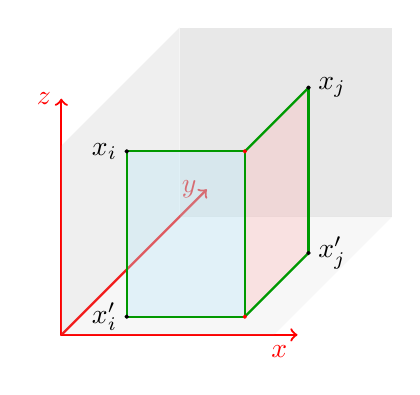
\begin{tikzpicture}[scale=0.30, line join=round, line cap=round]


\draw[->, thick, red] (0,0,13) -- (10,0,13) node[below left] {$x$};
\draw[->, thick, red] (0,0,13) -- (0,10,13) node[left] {$z$};
\draw[->, thick, red] (0,0,13) -- (0,0,-3) node[left] {$y$};


\coordinate (xi') at (2,0,11);
\coordinate (xj') at (7,0,4);
\coordinate (xi) at (2,7,11);
\coordinate (xj) at (7,7,4);


\coordinate (xip) at (7,7,11);
\coordinate (xjp) at (7,0,11);
%planes
\fill[black!30, opacity=0.111] (0,0,0)--(9,0,0)--(9,0,13) -- (0,0,13);
\fill[black!30, opacity=0.204] (0,0,0)--(0,8,0)--(0,8,13) -- (0,0,13);
\fill[black!30, opacity=0.3] (0,0,0)--(0,8,0)--(9,8,0)--(9,0,0);
% Draw the two parallelograms (sides of a prism)
\fill[cyan!30, opacity=0.313] (xi) -- (xi') -- (xjp) -- (xip) -- cycle;
\fill[red!30, opacity=0.313] (xj') -- (xj) -- (xip) -- (xjp) -- cycle;

% Edges

\draw[thick, green!60!black] (xj') -- (xjp);
\draw[thick, green!60!black] (xjp) -- (xip);
\draw[thick, green!60!black] (xjp) -- (xi');

\draw[thick, green!60!black] (xj) -- (xip);
\draw[thick, green!60!black] (xi) -- (xip);

% Vertical edges
\draw[thick, green!60!black] (xi') -- (xi);
\draw[thick, green!60!black] (xj') -- (xj);

% Red dots (middle edges between layers)
\filldraw[red] (xip) circle (2pt);
\filldraw[red] (xjp) circle (2pt);

% Nodes
\filldraw[black] (xi') circle (2pt) node[left] {$x_i'$};
\filldraw[black] (xi) circle (2pt) node[left] {$x_i$};
\filldraw[black] (xj') circle (2pt) node[right] {$x_j'$};
\filldraw[black] (xj) circle (2pt) node[right] {$x_j$};

\end{tikzpicture}
    \caption{\textbf{Case 1:} We simply replace,the pair \(x_i,x_j\) with \(x'_i,x'_j\) }
\end{figure}

    In each case we have chosen \(\lambda_\varepsilon\) in a way that, at both of the points \(x_i\) and \(x_j\) the projection cycle-vectors \((p,\lambda)\) and \((p_0,\lambda_\varepsilon)\) have weights with opposite signs. Thus, by the Lemma \ref{lemma-denominators}, for \(\varepsilon>0\) small enough, we have 
    \[
    0 < \sum_{}|\lambda'_i| \le  \sum|\lambda_i|,
    \]
where \((p',\lambda')=(p,\lambda)+(p_0,\lambda_\varepsilon)\).

On the other hand, applying the Lemma \ref{main-func-ineq} gives
\[
\sum_{x \in p'}\lambda'(x)f(x) \ge \sum_{x \in p}\lambda(x)f(x).
\]
Hence, in all three cases, we will get a contradiction to the optimality of \((p,\lambda)\) simultaneously as in part \((a)\).


\textbf{(c)} Let \((p,\lambda)=(x_0,x_1,...,x_m,\lambda_0,\lambda_1,...,\lambda_m)\) be an optimal projection cycle-vector for \(f\) on the set \(S\) that contains a point \(x_i=(\xi_i,\gamma_i,\zeta_i)\) with \(\lambda_i<0\).

Consider the planes \(x=\xi_i,y=\gamma_i\) and \(z=\zeta_i\). By the definition of the projection cycle, each of these planes contains at least one point of \(p\) with positive weight. Let these points be \(x_j=(\xi_i,\gamma_j,\zeta_j),x_l=(\xi_l,\gamma_i,\zeta_l),x_k=(\xi_k,\gamma_k,\zeta_i)\).
%with weights \(\lambda_j,\lambda_k,\lambda_l>0\) respectively. 
If any of these positive-weighted points makes a well-ordered pair with \(x_i\), then the projection cycle-vector \((p,\lambda)\) cannot be optimal by part \((b)\). 
\begin{figure}[ht]
        \centering
        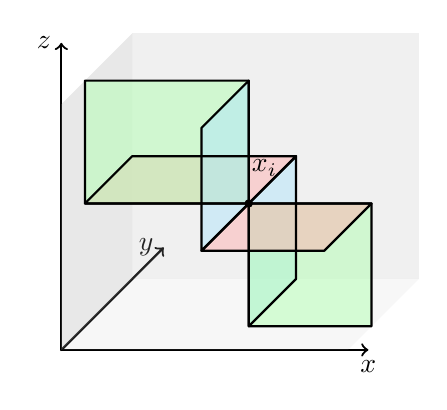
\begin{tikzpicture}[scale=0.26, line join=round, line cap=round]
% Axis
\draw[->, thick, black] (0,0,-3) -- (15,0,-3) node[below] {$x$};
\draw[->, thick, black] (0,0,-3) -- (0,15,-3) node[left] {$z$};
\draw[->, thick, black] (0,0,-3) -- (0,0,-16) node[left] {$y$};
%planes
\fill[black!30, opacity=0.1] (0,0,-3) -- (14,0,-3) -- (14,0,-12) -- (0,0,-12) -- cycle;
\fill[black!30, opacity=0.3] (0,0,-3) -- (0,12,-3) -- (0,12,-12) -- (0,0,-12) -- cycle;
\fill[black!30, opacity=0.2] (14,0,-12) -- (14,12,-12) -- (0,12,-12) -- (0,0,-12) -- cycle;

\coordinate (xi) at (8,6,-6);

\fill[cyan!30, opacity=0.513] (xi) -- (8,6,-12) -- (8,0,-12) -- (8,0,-6) -- cycle;
\fill[red!30, opacity=0.513] (xi) -- (8,6,-12) -- (0,6,-12) -- (0,6,-6) -- cycle;
\fill[green!30, opacity=0.513] (xi) -- (8,12,-6) -- (0,12,-6) -- (0,6,-6) -- cycle;
\fill[green!30, opacity=0.513] (xi) -- (8,0,-6) -- (14,0,-6) -- (14,6,-6) -- cycle;
\fill[cyan!30, opacity=0.513] (xi) -- (8,6,0) -- (8,12,0) -- (8,12,-6) -- cycle;
\fill[red!30, opacity=0.513] (xi) -- (8,6,0) -- (14,6,0) -- (14,6,-6) -- cycle;
%lines
\draw[thick, black!60!black] (xi) -- (8,6,-12) -- (8,0,-12) -- (8,0,-6) -- cycle;
\draw[thick, black!60!black] (xi) -- (8,6,-12) -- (0,6,-12) -- (0,6,-6) -- cycle;
\draw[thick, black!60!black] (xi) -- (8,12,-6) -- (0,12,-6) -- (0,6,-6) -- cycle;
\draw[thick, black!60!black] (xi) -- (8,0,-6) -- (14,0,-6) -- (14,6,-6) -- cycle;
\draw[thick, black!60!black] (xi) -- (8,6,0) -- (8,12,0) -- (8,12,-6) -- cycle;
\draw[thick, black!60!black] (xi) -- (8,6,0) -- (14,6,0) -- (14,6,-6) -- cycle;

% Nodes
\filldraw[black] (xi) circle (5pt) node[label={[xshift=0.20cm, yshift=0.1cm]{$x_i$}}]{};


\end{tikzpicture}
        \caption{The possible locations of the points that balances \(x_i\)} due to part \((b)\).
        \label{fig:(c)}
\end{figure}
 
Assume both \(0<\xi<1\) and \(0<\gamma<1\). By the part \((b)\) we have that \((x_i,x_j)\) is not a well-ordered pair,thus, either \(\gamma_i< \gamma_j, \zeta_i > \zeta_j\) or \(\gamma_i> \gamma_j, \zeta_i < \zeta_j\). Similarly, \((x_i,x_l)\) is not a well-ordered pair, thus, either \(\xi_i< \xi_l, \zeta_i > \zeta_l\) or \(\xi_i> \xi_l, \zeta_i < \zeta_l\). It is easy to verify that in each of the four possible cases, \(x_j,x_l\) cannot be a well-ordered pair. By part \((a)\) if \((p,\lambda)\) is optimal, then any pair of points \(x_j,x_l,x_k\) should be well-ordered. Thus, \((p,\lambda)\) cannot be optimal, and we get a contradiction.
Since we choose \(\xi,\gamma\) arbitrarily from \(\xi,\gamma,\zeta\), this contradiction works if at least two of the planes \(x=\xi_i,y=\gamma_i\) and \(z=\zeta_i\) are inner planes, which happens when \(x_i\) is not on the edges of the unit cube.
Hence, \(x_i\) belongs to one of the edges of the unit cube. 

Now, if, \(x_i\) and \((0,0,0)\) are on the same edge, we have three cases: \(x_i=(\xi,0,0)\) or \(x_i=(0,\gamma,0)\) or \(x_i=(0,0,\zeta)\). Assume that \(x_i=(\xi,0,0)\), then on the inner plane \(x=\xi\) there exist another point \(x_j=(\xi,\gamma_j,\zeta_j) \in p\) with \(\lambda_j>0\). Moreover, since \(\gamma_j,\zeta_j \ge 0\), \(x_i\) and \(x_j\) are well-ordered. But this contradicts the optimality of \((p,\lambda)\), by part \((b)\). Similarly, in the other two cases, we get a contradiction.

Using similar arguments, it can be proven that \(x_i\) and \((1,1,1)\) cannot be on the same edge.

Thus, \(x_i\) belongs to one of the edges of the cube, which does not contain any of the vertices \((0,0,0)\) and \((1,1,1)\).
Let's name these edges \(l_1,...,l_6\) as following 
\begin{align*}    
    l_1=\{(\xi,0,1), 0 \le \xi \le 1\}, \\
    l_2=\{(1,0,\zeta), 0 \le \zeta \le 1\},\\
    l_3=\{(1,\gamma,0), 0 \le \gamma \le 1\}, \\
    l_4=\{(\xi,1,0), 0 \le \xi \le 1\},\\
    l_5=\{(0,1,\zeta), 0 \le \zeta \le 1\}, \\
    l_6=\{(0,\gamma,1), 0 \le \gamma \le 1\}.\\
\end{align*}

\textbf{(d)}
    Assume the contrary, let \(x_i \in p\) be a point on one of the edges of the unit cube with \(\lambda_i>0\). We have three cases:
    \textbf{Case 1:} \(x_i\) is on the same edge with one of the vertices \((0,0,0)\) or \((1,1,1)\).\\
    If \(x_i\) and \((0,0,0)\) are on the same edge, have three cases: \(x_i=(\xi,0,0)\) or \(x_i=(0,\gamma,0)\) or \(x_i=(0,0,\zeta)\). Assume \(x_i=(\xi,0,0)\), then on the inner plane \(x=\xi\) there exists another point \(x_j=(\xi,\gamma_j,\zeta_j) \in p\) with \(\lambda_j<0\). Moreover, since \(\gamma_j,\zeta_j \ge 0\), \(x_i\) and \(x_j\) are well-ordered. But this contradicts the optimality of \((p,\lambda)\), by part \((b)\). 
    
    Similarly, in the other two cases, we get a contradiction.
    Using similar arguments, it can be proven that \(x_i\) and \((1,1,1)\) cannot be on the same edge.
    
    \textbf{Case 2:} \(x_i\) belongs to one of the edges of the cube, not containing any of the vertices \((0,0,0)\) and \((1,1,1)\). Without loss of generality, we can assume that \(x_i=(\xi,0,1)\). To make the sum of weights on the plane \(z=1\) equal to zero, there should exist a point \(x_j\) of \(p\) with a negative weight on \(z=1\). By part \((c)\) the point \(x_j\) belongs to at least one of the edges \(l_1\) or \(l_6\). Thus, we have two sub-cases:
    
    \textbf{Case 2.1:} \(x_j=(\xi_j,0,1)\) for some \(0 \le \xi_j \le 1\).  Clearly, \(\xi_j \ne \xi\). We should consider two sub-cases:
    
    \textbf{Case 2.1.1:} \(\xi_j < \xi\)\\
    Consider the projection cycle \((p, \lambda_\varepsilon)\), where \(p_0=(x_i, x_j, (\xi,1,1), (\xi_j,1,1))\) and \(\lambda_\varepsilon=(-\varepsilon,\varepsilon,\varepsilon,-\varepsilon)\);
    
    \textbf{Case 2.1.2:} \(\xi < \xi_j\)\\
    Consider the projection cycle \((p_0, \lambda_\varepsilon)\), where \(p_0=(x_i, x_j, (\xi,0,0), (\xi_j,0,0))\) and \(\lambda_\varepsilon=(\varepsilon,-\varepsilon,-\varepsilon,\varepsilon)\).

    Similarly to part \((a)\) and part \((b)\), taking \((p',\lambda')=(p,\lambda)+(p_0,\lambda_\varepsilon)\) we get a contradiction to the optimality of \((p,\lambda)\).
    
    \textbf{Case 2.2:} \(x_j=(0,\gamma,1)\) for some \(0 < \gamma \le 1\). 
    Consider the plane, \(y=\gamma\). To make the sum of weights on the plane \(y=\gamma\) equal to zero, there should exist a point \(x_k\) of \(p\) with a positive weight on \(y=\gamma\). Let \(x_k=(\xi_k,\gamma,\zeta)\). If \(\zeta=1\), the points \(x_j\) and \(x_k\) belonging to the inner plane \(y=\gamma\) becomes well-ordered and since \(x_j\) and \(x_k\) have opposite weights we get a contradiction by part \((b)\). If, \(\zeta<1\), the points, \(x_i\) and \(x_k\) becomes non well-ordered. Since both of \(x_i\) and \(x_k\) have positive weights, we get a contradiction by the part \((a)\).
    \\
    Since we get a contradiction in each case, the proof of part \((d)\) is completed.


\textbf{(e)} 
    Consider the point \(x_i=(\xi_i,\gamma_i,\zeta_i)\in p\) with minimal coordinates among the positive weighted points of \(p\). (Since the positive weighted points are well-ordered pairwise, the point with the minimal sum of coordinates has minimal coordinates.) 
    
    If \(x_i=(0,0,0)\), we are done. Otherwise, since \(x_i\) is chosen to be minimal, it cannot be any other vertex of the unit cube, and thus there is at least one inner plane passing through \(x_i\). 
    Without loss of generality, assume that this plane has equation \(x=\xi_i\). Then, on the plane \(x=\xi_i\) there is another point \(x_j=(\xi_i,\gamma_j,\zeta_j) \in p\) such that \(\lambda_j<0\). By part \((b)\) we know that \(x_i\) and \(x_j\) cannot be well-ordered, and hence, either \(\gamma_j<\gamma_i\) or \(\zeta_j<\zeta_i\) but in the first case on the plane \(y=\gamma_j\) and in the second case on the plane \(z=\zeta_j\) there is a positive weighted point to make the sum over that plane equal to zero. But this contradicts to the minimality of \(x_i\) and, hence, \(x_i=(0,0,0)\).

    Similarly, we can prove that the positive weighted point with maximal coordinates is \((1,1,1)\).

%\end{enumerate}
\begin{figure}[ht]
\centering
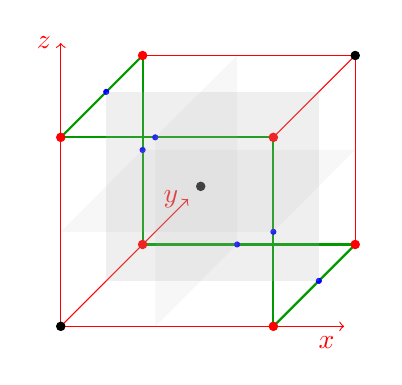
\begin{tikzpicture}[scale=0.3, line join=round, line cap=round]
% Axis
\draw[->, red] (0,0,9) -- (12,0,9) node[below left] {$x$};
\draw[->, red] (0,0,9) -- (0,12,9) node[left] {$z$};
\draw[->, red] (0,0,9) -- (0,0,-5) node[left] {$y$};

\coordinate (T_4) at (9,8,0);
\coordinate (T_3) at (0,8,0);
\coordinate (T_2) at (9,0,0);
\coordinate (T_1) at (0,0,0);
\coordinate (T_5) at (9,8,9);
\coordinate (T_6) at (0,8,9);
\coordinate (T_7) at (9,0,9);
\coordinate (T_8) at (0,0,9);
\coordinate (T_x) at (4,4,4);
\coordinate (T_y) at (2,3,3);
\coordinate (T_z) at (7,6,7);

% intersection (z-direction)
\coordinate (xip) at (7,7,11);
\coordinate (xjp) at (7,3,11);

\draw[thick, green!60!black] (T_1) -- (T_2);
\draw[thick, green!60!black] (T_1) -- (T_3);
\draw[thick, green!60!black] (T_3) -- (T_6);
\draw[thick, green!60!black] (T_6) -- (T_5);
\draw[thick, green!60!black] (T_5) -- (T_7);
\draw[thick, green!60!black] (T_7) -- (T_2);
\draw[red] (T_4) -- (T_3);
\draw[red] (T_4) -- (T_5);
\draw[red] (T_4) -- (T_2);

\filldraw[red] (T_1) circle (5pt) node[right] {};
\filldraw[red] (T_2) circle (5pt) node[right] {};
\filldraw[red] (T_3) circle (5pt) node[right] {};
\filldraw[black] (T_4) circle (5pt) node[right] {};
\filldraw[red] (T_5) circle (5pt) node[right] {};
\filldraw[red] (T_6) circle (5pt) node[right] {};
\filldraw[red] (T_7) circle (5pt) node[right] {};
\filldraw[black] (T_8) circle (5pt) node[right] {};
\filldraw[black] (T_x) circle (5pt) node[right] {};
\filldraw[blue] (9,0,4) circle (3pt) node[right] {};
\filldraw[blue] (4,0,0) circle (3pt) node[right] {};
\filldraw[blue] (0,8,4) circle (3pt) node[right] {};
\filldraw[blue] (0,4,0) circle (3pt) node[right] {};
\filldraw[blue] (4,8,9) circle (3pt) node[right] {};
\filldraw[blue] (9,4,9) circle (3pt) node[right] {};
%\filldraw[black] (T_y) circle (5pt) node[right] {};
%\filldraw[black] (T_z) circle (5pt) node[right] {};
\fill[black!30, opacity=0.111] (4,0,0)--(4,8,0)--(4,8,9)--(4,0,9);
\fill[black!30, opacity=0.211] (9,0,4)--(9,8,4)--(0,8,4)--(0,0,4);
\fill[black!30, opacity=0.11] (0,4,0)--(0,4,9)--(9,4,9)--(9,4,0);
\end{tikzpicture}
         \label{f:Lemma 2.2}
         \caption{Geometric interpretation: Theorem 2.2}
\end{figure}

\end{proof} 

\end{document}
